\chapter{Configuration} % Titlul capotilului
\label{Capitolul3}

\section{Introduction}

The applications in the ATLAS TDAQ system register up to several thousands of objects that represent information to be monitored. Different objects need to be published in different ways: for example with different publishing frequency and or to different Information Sharing (IS) servers or even need to be written to a file. As an example, the number of failed checksums of the event data read from the detector needs to be published every 10 seconds to an IS server called "L1". For another example, the histogram of accepted event data size should be written to a file called "DF.root" at the end of the running period. We aim to provide a way for the user to specify these parameters in an expressive, succinct and easy to use way. This process is called the \emph{configuration} of the library.

\section{Requirements}

The library allows the user to specify one or multiple \emph{publishing targets}. The publishing targets currently include IS servers, OH servers, files in ROOT format and standard output. For each target, the user can specify some \emph{publishing parameters}, for example, the name of the IS server and the publishing interval for an IS publishing target.

Another important functionality is to be able to modify the configuration at runtime. For example, if an operator notices some abnormal conditions in the running of the system, she may enable some debug monitoring information to be published in order to identify and fix the problem. 

\section{Challenges}

As with other parts of the system, the main challenge of the configuration is the scale of the system. We discuss below how each dimension of scaling impacts the design of the library.

\subsection*{The code size}

First of all, in order to publish a monitored object, the library needs to know the publishing parameters. The first decision to be made is whether to associate the parameters with the objects programmatically (in the source code), or in an external file which is loaded at runtime. We chose the second approach since, any change in the source code requires a recompilation and to create a binary patch of the current release version of the software. The duration and complexity of this process would discourage developers from changing configurations. In the external file approach, a change in configuration can be as simple as editing a text file and checking it in in the source repository.

\subsection*{The number of monitored objects}

With over 5000 monitored objects, we need to keep the configuration file of an application within a manageable size. We leverage the fact that the objects fall into a few semantic categories that share publishing requirements. We define groups of objects that share the same publishing parameters by using regular expressions. 

\begin{figure}[ht]
\centering
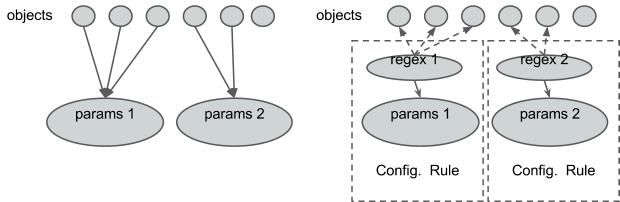
\includegraphics[scale=0.6]{../Images/oks_regex.png}
\caption[Publishing parameters association.]{The two approaches for associating publishing parameters with monitored objects: explicit (left) and implicit by using regular expressions (right).}
\label{fig:oks_regex}
\end{figure}

As presented in the figure \ref{fig:oks_regex}, instead of having explicit links from the monitored objects to sets of parameters, we create links from parameters to objects by using configuration rules. A configuration rule is composed of a regular expression and a set of parameters. It is this rules that we store in the configuration file. A nice side-effect of this approach is that if the programmer registers a new object which uses an existing parameter set, she just has to give it a name that matches the regular expression.

One problem related to the object sets specification as regular expressions is that it is not easy to express exceptions from a rule. For example: we want to publish histograms with names matching {\tt “DEBUG/.*”} every 10 seconds, but we have a really big histogram among them that we would like to publish less often. To this end, we chose to add an exclude filter to every configuration rule that specifies the exceptions to that rule.

\subsection*{The number of developers}

In order to avoid complicated link time dependencies between packages, we adopted the split responsibility model: the developer of a library (other than {\tt monsvc}) registers some objects and the developer of the application (which uses the library) is the one who needs to configure their publishing parameters. Since some objects are registered by one developer and configured by another one, a clear convention should be used between the two. 

Our configuration mechanism allows the library developer to provide configuration rules for the objects registered by its library. To this end we created the concept of rule bundle which contains configuration rules and links other rule bundles. With this approach the developer of the main application can just link the rule bundle of the library from the rule bundle of the application. This mechanism handles nicely transitive dependencies by using transitively linked bundles.

The configuration files are a set of interlinked XML files, one per application or library. These files form the configuration database which can be loaded at run time by using the OKS system. The database is an object oriented one, where for example every application is described by a {\tt PublishingApplication} object which has a one to one relation to a rule bundle which is represented by an object of class {\tt ConfigurationRuleBundle}. The complete schema of the configuration database is presented in figure \ref{fig:oks_schema}. 

\begin{figure}[ht]
\centering
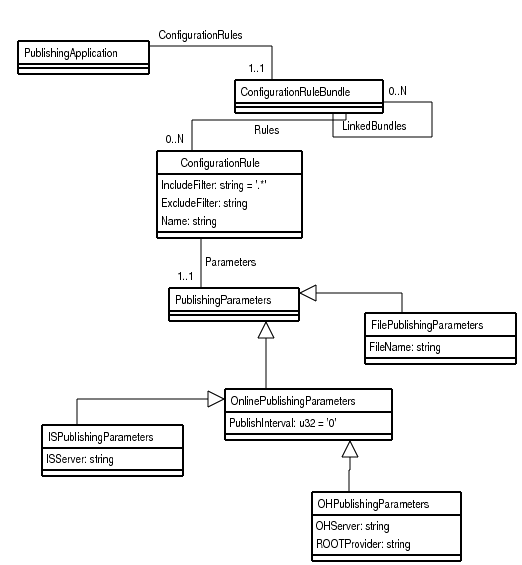
\includegraphics[scale=0.75]{../Images/oks_schema.png}
\caption{Configuration database schema.}
\label{fig:oks_schema}
\end{figure}

\subsection*{The number of application instances}

Some applications in our system have several thousands of instances which use similar configuration files with only a few configuration parameters that differ. For example, if every application writes the objects in a file, then the name of the file should be different for the applications running on the same node. These configuration files are generated automatically from a common template using the partition editor tool.

Another challenge is related to the configuration changes during a running period. Our solution uses IS commands mechanism to allow the human operator to send the configuration change commands to the IS server which forwards them to the applications.